\documentclass[border = 1.5cm]{standalone}
%%%% packages
\usepackage{tikz}
\usetikzlibrary{trees, arrows, shapes.geometric, positioning} % TikZ libraries
%%%% layers
\pgfdeclarelayer{bg1}    % declare background layer
\pgfdeclarelayer{bg2}
\pgfsetlayers{bg2,bg1,main}  % set the order of the layers (main is the standard layer)

%%%% styles
\tikzset{
	every rectangle node/.style = {thick,anchor=west},
	io/.style = {rectangle, minimum width = 4cm, minimum height = 3cm, text centered, draw = black, fill = blue!10},
	main/.style = {rectangle, draw = black, rounded corners, minimum width = 3cm, minimum height = 1.25cm, text centered},
	ids/.style = {diamond, minimum width = 3cm, minimum height = 2cm, text centered, draw = black, fill = green!30},
	res/.style = {rectangle, rounded corners, minimum width = 2cm, minimum height = 1cm, text centered, draw = black, fill = blue!30},
	resvariables/.style = {rectangle, minimum width = 2cm, minimum height = 1cm, text centered},
	steps/.style = {rectangle, minimum width = 1cm, text centered, fill = yellow},
	arrow/.style = {->, > = stealth, draw = black, color = gray!80, line width = 3pt}
}

\begin{document}
	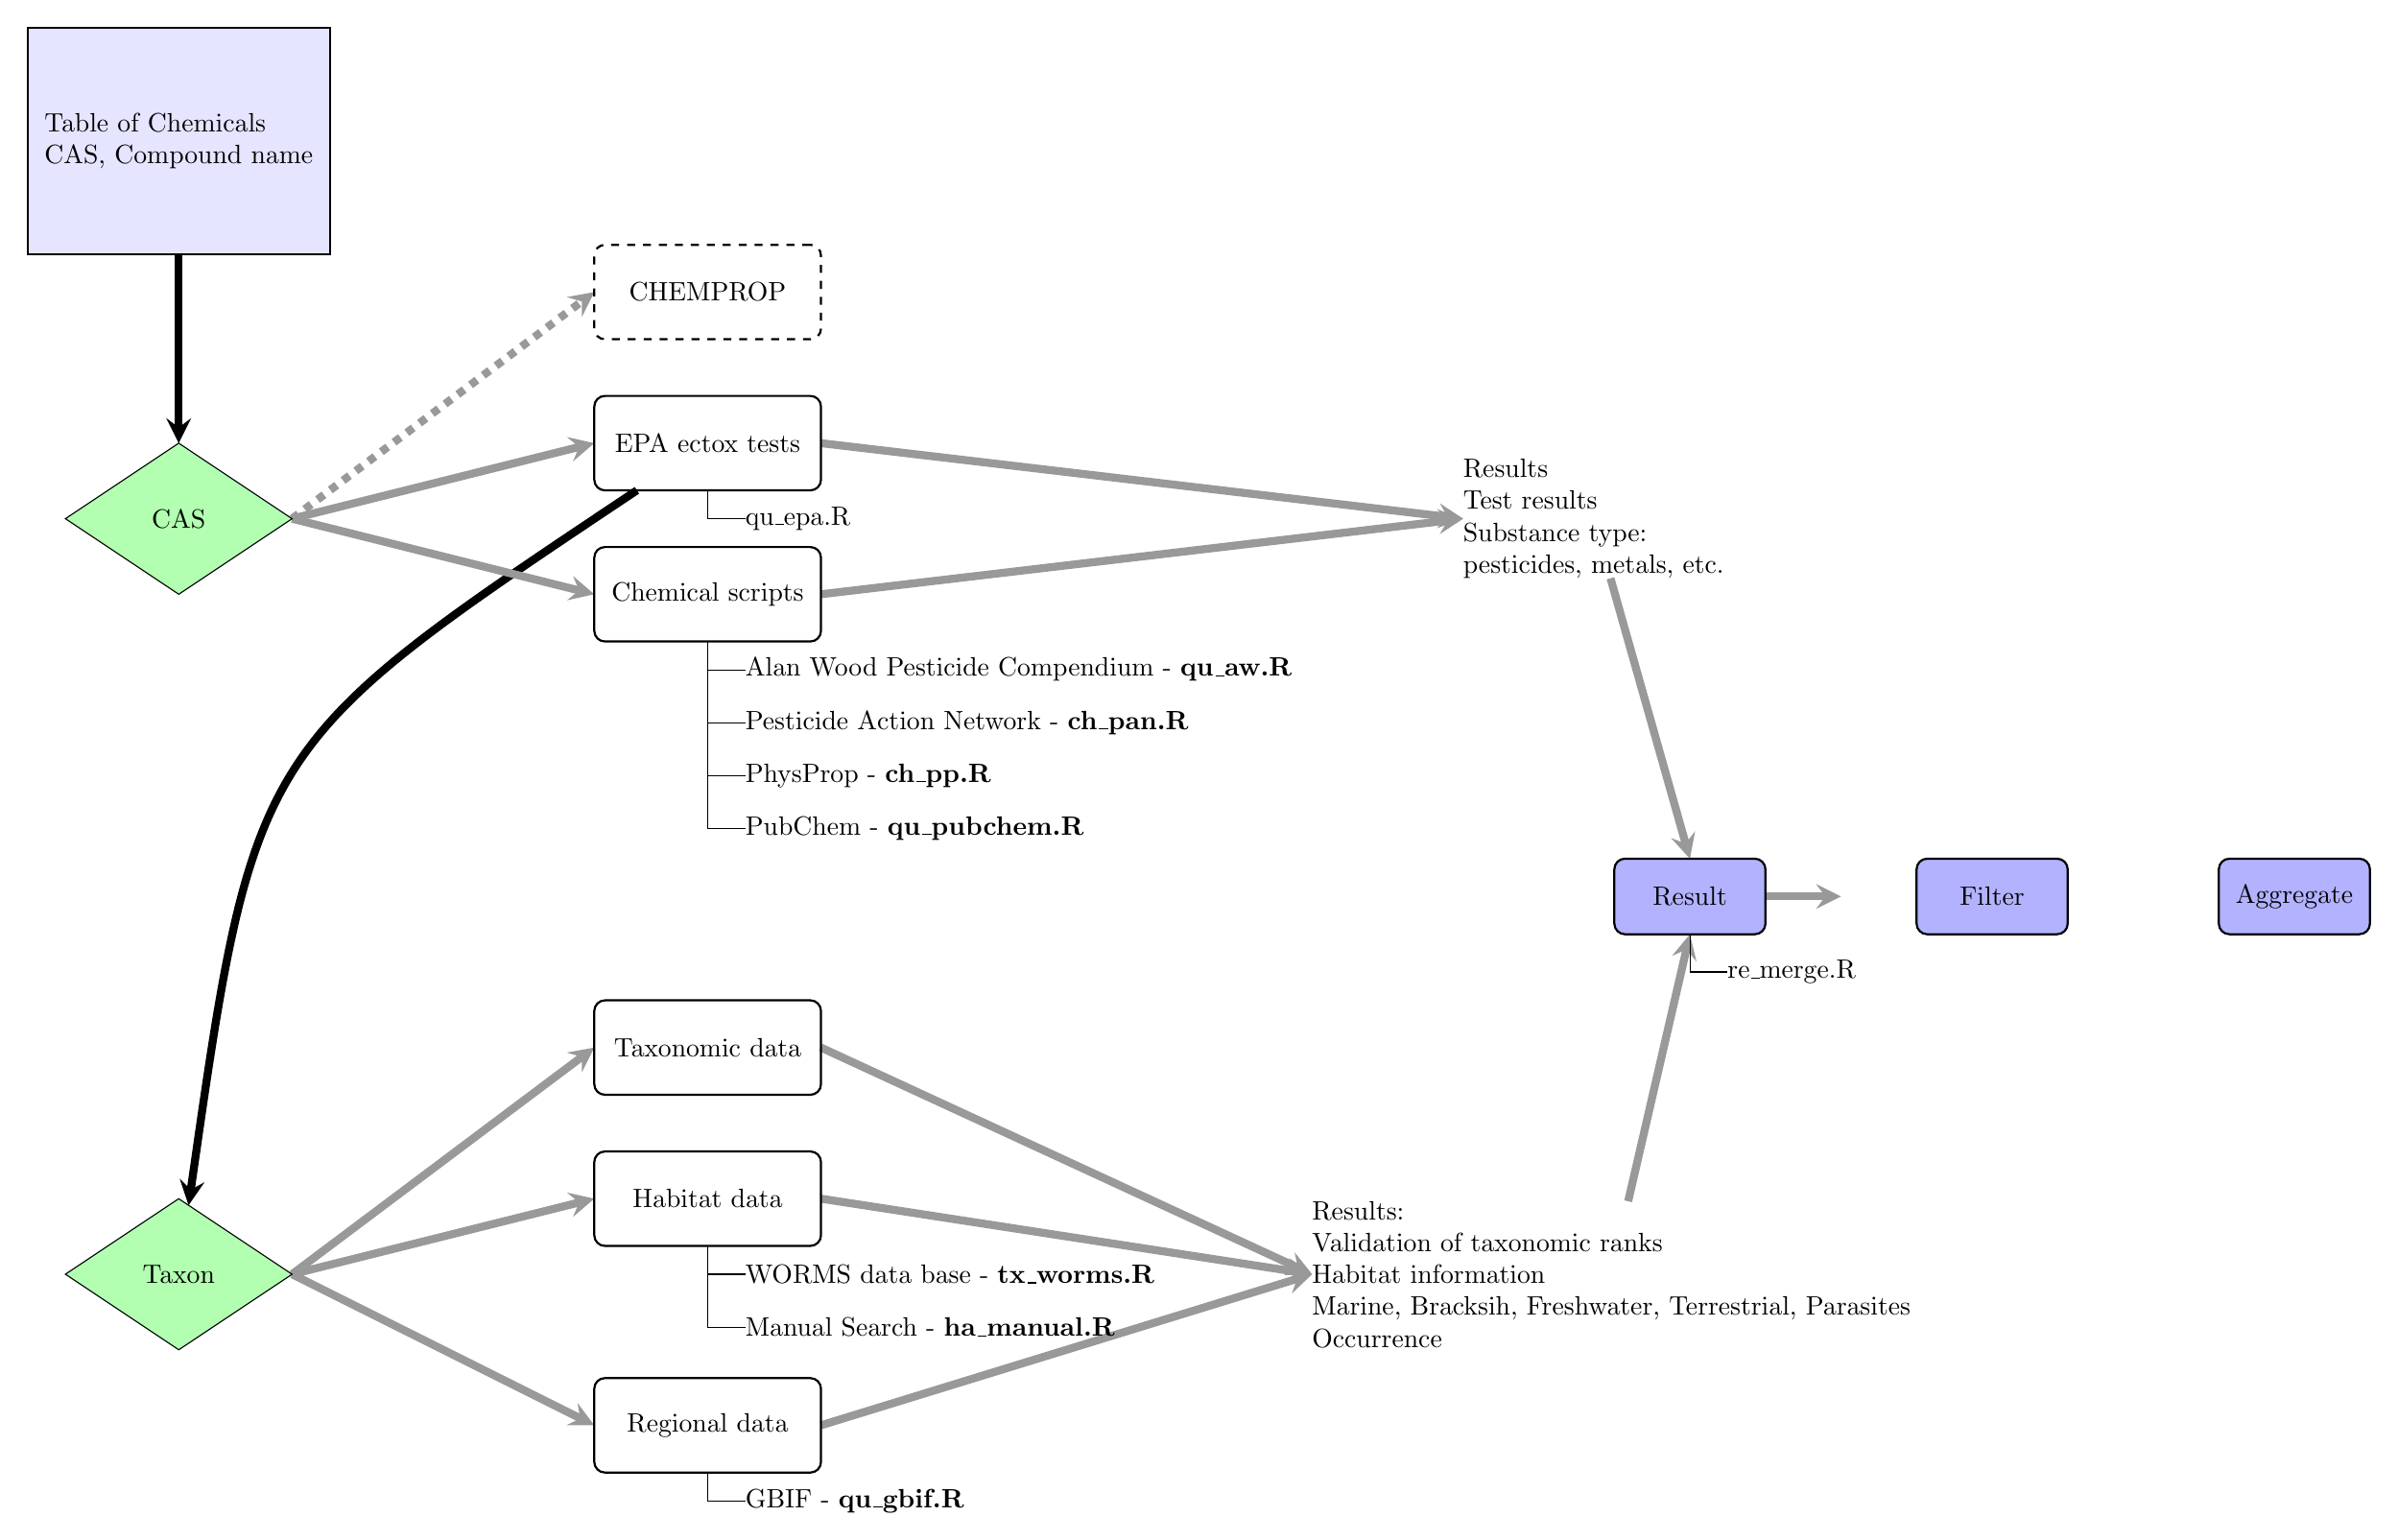
\begin{tikzpicture}[
	grow via three points={one child at (0.5,-1) and
		two children at (0.5,-1) and (0.5,-1.7)},
	edge from parent path={(\tikzparentnode.south) |- (\tikzchildnode.west)},
	inner sep = 0pt, outer sep = 0pt
	]
	
		\node (io) [io, align = left] at (0cm,0cm) {Table of Chemicals \\ CAS, Compound name};
		%% chemicals
		% id nodes


		\node (cas) [ids, below of=io, yshift = -4cm] {CAS};


		% main nodes
		\node (chemprop) [main, dashed, right of=cas, xshift=4.5cm, yshift=3cm] {CHEMPROP};
		\node (epa) [main, right of=cas, yshift=1cm, xshift=4.5cm] {EPA ectox tests}
			child { node { qu\_epa.R} };
		\node (chemscr) [main, right of=cas, yshift=-1cm, xshift=4.5cm] {Chemical scripts}
			child { node { Alan Wood Pesticide Compendium - \textbf{qu\_aw.R } }}
			child { node { Pesticide Action Network - \textbf{ch\_pan.R} }}
			child { node { PhysProp - \textbf{ch\_pp.R} }}
			child { node { PubChem - \textbf{qu\_pubchem.R} }};
		% result nodes
		\node (toxres) [resvariables, right of=cas, yshift=0cm, xshift=16cm, align = left] {Results\\Test results\\Substance type:\\pesticides, metals, etc.}; % result
		%\includegraphics{/home/andreas/Documents/Projects/etox-base/data/pubchemlogo2017.png};
	
		%\animategraphics{https://cfpub.epa.gov/ecotox/epafiles/images/logo_epaseal.gif}
		
		%% organisms
		% id nodes
		\node (taxon) [ids, below of=cas, yshift=-9cm, align = center] {Taxon}; % \\ {(Genus or Species)}}; % escape brackets usin curly brackets
		% main nodes
		\node (taxonquery) [main, right of=taxon, xshift = 4.5cm, yshift = 3cm] {Taxonomic data};
		\node (habitat) [main, right of=taxon, xshift = 4.5cm, yshift = 1cm] {Habitat data}
			child { node { WORMS data base - \textbf{tx\_worms.R} }}
			child { node { Manual Search - \textbf{ha\_manual.R} }};
		\node (region) [main, right of = taxon, xshift = 4.5cm, yshift = -2cm] {Regional data}
			child { node { GBIF - \textbf{qu\_gbif.R} }};
		% result nodes
		\node (taxres) [resvariables, right of=taxon, xshift = 14cm, align = left] {Results:\\Validation of taxonomic ranks\\Habitat information\\Marine, Bracksih, Freshwater, Terrestrial, Parasites\\Occurrence}; % result
		
		%% final result
		\node (testres) [res, right of = cas, xshift = 18cm, yshift = -5cm] {Result}
			child { node { re\_merge.R} };
		\node (filtres) [res, right of = testres, xshift = 2cm] {Filter};
		\node (aggres) [res, right of = filtres, xshift = 2cm] {Aggregate};

		%%% arrows %%%
		\begin{pgfonlayer}{bg1}
		\draw [arrow, black] (io) -- (cas);
		\draw [arrow, dashed] (cas.east) -- (chemprop.west);
		\draw [arrow] (cas.east) -- (chemscr.west);
		\draw [arrow] (cas.east) -- (epa.west);
		\draw [arrow] (epa.east) -- (toxres.west);
		\draw [arrow] (chemscr.east) -- (toxres.west);
		
%		\draw [arrow] (epa.east) -| (testres.north);
%		\draw [arrow] (chemscr.east) -| (testres.north);
		
		%\begin{scope}[on background layer]
		\begin{pgfonlayer}{bg2}
			\draw [arrow, black] (epa) .. controls (3cm,-8cm) .. (taxon);
		\end{pgfonlayer}
		%\end{scope}
		
		\draw [arrow] (taxon.east) -- (habitat.west);
		\draw [arrow] (taxon.east) -- (region.west);
		\draw [arrow] (taxon.east) -- (taxonquery.west);
		\draw [arrow] (habitat.east) -- (taxres.west);
		\draw [arrow] (taxonquery.east) -- (taxres.west);
		\draw [arrow] (region.east) -- (taxres.west);
		\draw [arrow] (toxres) -- (testres.north);
		\draw [arrow] (taxres) -- (testres.south);
		
		\draw [arrow, right of = testres] (testres) -- ++(2cm,0cm);
	
		\end{pgfonlayer}
	\end{tikzpicture}
\end{document}